\documentclass[portrait]{a0poster}
\usepackage[T1]{fontenc}

\usepackage[english]{babel} % langue utilisée

% \usepackage{lmodern} % For times font (times)
\renewcommand{\familydefault}{\sfdefault}
\usepackage[scaled]{helvet}

\usepackage{titlesec} % pour de plus beaux titres ?
\usepackage{amsmath} %,amsfonts,amsmath,amssymb,amsthm % symboles mathématiques

\usepackage{multicol} % multiples colonnes
\usepackage{float} % float environnement
\usepackage[svgnames]{xcolor} % plus de couleurs
\usepackage{tcolorbox}

\usepackage{graphicx} % add figures and images
\usepackage{caption}
\graphicspath{{./fig/} } % image and figure path
\usepackage{tikz} % pour les graphiques
\usepackage{exscale} % ordre de mesures...

\usepackage[
    sorting=none,
    doi=false,
    url=false,
    isbn=false
]{biblatex} % bibliographie
\AtEveryBibitem{\clearlist{language}}
\addbibresource{biblio.bib}
\def\bibfont{\small}

%% Reformatage du fichier
\usepackage[left=1cm,right=1cm,top=1cm,bottom=1cm]{geometry}
\setlength{\paperwidth}{84.1cm}	% Poster width in cm
\setlength{\paperheight}{118.9cm}	% Poster height in cm
\setlength{\textwidth}{80.1cm}
\setlength{\textheight}{114.9cm}

%% Reformatage des tailles de titre
\titleformat*{\section}{\LARGE\bfseries}
\titleformat*{\subsection}{\Large\bfseries}
\titleformat*{\subsubsection}{\large\bfseries}
\titleformat*{\paragraph}{\large\bfseries}

% %%%%%%%%%%%%%%%%%%%%%%%%%%%%%%%%%%%%%
% %         Début Document            %
% %%%%%%%%%%%%%%%%%%%%%%%%%%%%%%%%%%%%%

\begin{document}
    \vspace{1cm}

    \begin{minipage}{\textwidth}
        \begin{minipage}{0.65\textwidth}
            \textbf{\Huge Population decoding of visual motion direction.} \vspace{1cm} \\
            \textbf{\large Alexandre Lainé *¹,  Nicholas J. Priebe ², Guillaume S. Masson ¹, Laurent U. Perrinet ¹} \\
            \large ¹ Institut de Neurosciences de la Timone, UMR 7289, CNRS and Aix-Marseille Université, Marseille, 13005, France.\\ 
            \large ² Section of Neurobiology, School of Biological Sciences, University of Texas at Austin, Austin, TX, USA.\\ 
            \large * Correspondence : alexandre.laine@univ-amu.fr
        \end{minipage}
        \hfill
        \begin{minipage}{0.35\textwidth}
            \begin{minipage}{0.48\textwidth}
                
\includegraphics[width=1\textwidth]{LogoAmidex.png} \\
                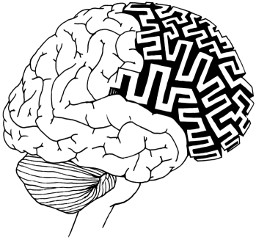
\includegraphics[width=0.35\textwidth]{LogoAREADNE.jpg}
                
\includegraphics[width=0.6\textwidth]{LogoAMU.pdf}
            \end{minipage}
            \hfill
            \begin{minipage}{0.48\textwidth}
                
\includegraphics[width=1\textwidth]{LogoINT.pdf}
            \end{minipage}
        \end{minipage}
    \end{minipage}

    \vspace{1cm}

    % \begin{minipage}{\textwidth}
    %     %%%%%%%%%%%%%%%%
    %     % INTRODUCTION %
    %     \begin{minipage}{0.4\textwidth}    
    %         \begin{tcolorbox}[
    %             title=\textbf{\Large{Introduction}}, 
    %             colframe=blue!60!black!,
    %             colback=white, 
    %             boxsep=10mm
    %         ]
    %             \begin{minipage}{\textwidth}
    %                 Studying the \textbf{internal representation} of natural features (fig. \ref{fig:mc_and_natural_features}) in the primary visual cortex (V1), like direction or spatial frequency, is crucial to understand how we perceive the external world. Research on 2D motion direction in \textbf{non-human primates}~\cite{Hubel_Wiesel_1968, Berens_Ecker_Cotton_Ma_Bethge_Tolias_2012} in particular when displaying  \textbf{naturalistic stimuli} like MotionClouds~\cite{Leon_Vanzetta_Masson_Perrinet_2012} reveals substantial diversity and multiple mechanisms within the neuronal population~\cite{Ladret_Cortes_Ikan_Chavane_Casanova_Perrinet_2023} (fig. \ref{fig:subpopulations}). The aim of this project is to examine how a large population of V1 neurons encodes stimulus direction and how this representation is modulated by the uncertainty using \textbf{decoding methods}. \\
    %             \end{minipage}

    %             \begin{minipage}{0.48\textwidth}
    %                 \begin{center}
    %                     \includegraphics[width=\textwidth]{intro_fig.pdf}   
    %                     \captionof{figure}{Uncertainty in natural images and MotionClouds.}
    %                     \label{fig:mc_and_natural_features}
    %                 \end{center}
    %             \end{minipage}
    %             \hfill
    %             \begin{minipage}{0.48\textwidth}
    %                 \begin{center}
    %                     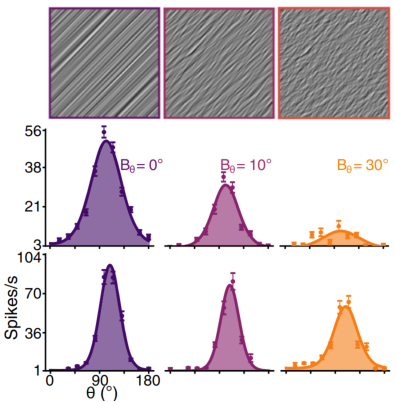
\includegraphics[width=\textwidth]{two_subpopulation_cats.pdf}
    %                     \captionof{figure}{Two subpopulation in cats area 17 (from~\cite{Ladret_Cortes_Ikan_Chavane_Casanova_Perrinet_2023}).}
    %                     \label{fig:subpopulations}
    %                 \end{center}
    %             \end{minipage}
    %         \end{tcolorbox}

    %         \vspace{1.5cm}

    %         \begin{tcolorbox}[
    %             title=\textbf{\Large{Acknowledgements}}, 
    %             colframe=gray!60!black!,
    %             colback=white, 
    %             boxsep=10mm
    %         ]
    %             This work was supported by ANR-NSF CRCNS grant “PrioSens” N° ANR-20-NEUC-0002 attributed to G.S.M, N.J.P. and L.U.P. and by a doctoral grant from the French Ministry of Higher Education and Research, awarded by the Doctoral School 62 of Aix-Marseille University to A.L.
    %         \end{tcolorbox}
    %     \end{minipage}
    %     \hfill
    %     %%%%%%%%%%%
    %     % METHODS %
    %     \begin{minipage}{0.58\textwidth}
    %         \begin{tcolorbox}[
    %             title=\textbf{\Large{Methods}},
    %             colback=white, 
    %             colframe=red!60!black,
    %             boxsep=10mm
    %         ]
    %             \begin{minipage}{0.4\textwidth}
    %                 Neuronal recordings (fig.~\ref{fig:spiking}) were made in V1 of one marmoset monkey using the Neuropixel 1.0 technology~\cite{Jun_Steinmetz_Siegle_Denman_Bauza_Barbarits_Lee_Anastassiou_Andrei_Aydın_et_al._2017} during 2D motion presentation in eight directions ($\theta$) from $0^{\circ}$ to $375^{\circ}$ and two precision levels ($B_\theta$, high : $22^{\circ}$ or low : $90^{\circ}$). The decoding method (fig.~\ref{fig:decoding}) optimizes the weights of a multinomial logistic regression to achieve optimal decoding accuracy on a training set. \\
    %                 The objective is to decode the direction of the motion for each precision level. The training is conducted \textbf{(1)} on a broad time-window at the begining or the end of the stimulus presentation, \textbf{(2)} by applying temporal generalization~\cite{King_Dehaene_2014} or \textbf{(3)} after reducing dimensionality with dPCA~\cite{Kobak_Brendel_Constantinidis_Feierstein_Kepecs_Mainen_Qi_Romo_Uchida_Machens_2016}. All the results presented here are computed on the testing test. \\
    %             \end{minipage}
    %             \hfill
    %             \begin{minipage}{0.58\textwidth}
    %                 \includegraphics[width=1\textwidth]{activity_recorded.pdf}
    %                 \captionof{figure}{Spiking activity induced by one stimulus ($sf = 0.7~c/^{\circ}$, $B_{sf} = 0.175~c/^{\circ}$, $spd = 2~^{\circ}/s$, $\theta = 45~^{\circ}$, $B_\theta = 90~^{\circ}$)}
    %                 \label{fig:spiking}
    %             \end{minipage}
                
    %             \begin{center}
    %                 \includegraphics[width=1\textwidth]{decoding_methods.pdf}
    %                 \captionof{figure}{Decoding method implemented in Python3 using the PyTorch library.}
    %                 \label{fig:decoding}
    %             \end{center}
    %         \end{tcolorbox}
    %     \end{minipage}
        
    %     \vspace{1.3cm}
        
    %     \begin{minipage}{\textwidth}
    %         \begin{tcolorbox}[
    %             title=\textbf{\Large{Results}},
    %             colback=white, 
    %             colframe=green!60!black,
    %             boxsep=10mm
    %         ]
    %             \begin{minipage}{0.30\textwidth}
    %                 \begin{center}
    %                     \includegraphics[width=\textwidth]{raw_accuracy.pdf}
    %                     \captionof{figure}{Decoding results after training (left) on the begining of the evocked activity or (right) on the end for two precision level ($B_\theta$).}
    %                     \label{fig:accuracy_raw}
    %                     \vspace{1cm}
    %                     \includegraphics[width=\textwidth]{raw_tc_neuron0.pdf}
    %                     \includegraphics[width=\textwidth]{raw_tc_neuron31.pdf}
    %                     \includegraphics[width=\textwidth]{raw_tc_neuron32.pdf}
    %                     \captionof{figure}{Weights learned for three neurons (n° $0$, $31$, $32$).}
    %                     \label{fig:raw_tc}
    %                 \end{center}
    %             \end{minipage}
    %             \hspace{0.5cm}
    %             \begin{minipage}{0.30\textwidth}
    %                 \begin{center}
    %                     \includegraphics[width=\textwidth]{dpca_decomposed_accuracy.pdf}
    %                     \captionof{figure}{Decoding results after training (left) on the begining or (right) on the end of the time course of dPCA components for two precision level ($B_\theta$).}
    %                     \label{fig:accuracy_dpca}
    %                     \vspace{1cm}
    %                     \includegraphics[width=\textwidth]{dpca_decomposed_tc_neuron0.pdf}
    %                     \includegraphics[width=\textwidth]{dpca_decomposed_tc_neuron1.pdf}
    %                     \includegraphics[width=\textwidth]{dpca_decomposed_tc_neuron2.pdf}
    %                     \captionof{figure}{Weights learned for three components (n° $0$, $1$, $2$).}   
    %                     \label{fig:dpca_tc}
    %                 \end{center}
    %             \end{minipage}  
    %             \hspace{0.5cm}
    %             \begin{minipage}{0.39\textwidth}
    %                 \begin{center}
    %                     \includegraphics[width=\textwidth]{raw_tempgen.pdf}
    %                     \captionof{figure}{Temporal generalisation of the direction based on neuronal activity for two level of precision ($B_\theta$).}
    %                     \label{fig:tempgen_raw}
    %                     \hfill
    %                     \includegraphics[width=\textwidth]{dpca_decomposed_tempgen.pdf}
    %                     \captionof{figure}{Temporal generalisation of the direction based on dPCA components for two level of precision ($B_\theta$).}
    %                     \label{fig:tempgen_dpca}
    %                 \end{center}
    %             \end{minipage}
    %         \end{tcolorbox}
    %     \end{minipage}
    % \end{minipage}
    
    % \vspace{1.3cm}
    
    % \begin{minipage}{\textwidth}
    %     \begin{minipage}{0.4\textwidth}
    %         \begin{tcolorbox}[
    %             title=\textbf{\Large{Discussion}},
    %             colback=white, 
    %             colframe=blue!60!black,
    %             boxsep=10mm
    %         ]
    %         This decoding approach clarifies the \textbf{representation of directional information} in the marmoset primary visual cortex, its stability accross time and its modulation by the precision level (fig.~\ref{fig:accuracy_raw} and \ref{fig:tempgen_raw}). The existence of transient and sustained representations may support distinct functional roles for differents cortical layers~\cite{Ladret_Cortes_Ikan_Chavane_Casanova_Perrinet_2023,Ringach_Shapley_Hawken_2002}. Demixed principal component analysis allows us to reduce the dimension, work in a \textbf{neural state space} and filter the raw activity. This transformation improve the decoding accuracy (fig.~\ref{fig:accuracy_dpca} and \ref{fig:tempgen_dpca}) and improve the decoder's ability to generalise between time steps. Overall, this analysis shows qualitatively the existence of a \textbf{stable representation} of the information wich is modulated by the precision level of the stimulus.
    %         \end{tcolorbox}
    %     \end{minipage}
    %     \hfill
    %     \begin{minipage}{0.58\textwidth}
    %         \printbibliography[title=\textbf{\Large{References}}]
    %     \end{minipage}
    % \end{minipage}
\end{document}